% =========================================================
% CHAPTER 3
% =========================================================

\chapter{Phân tích yêu cầu hệ thống}
\label{Chapter3}

% =========================================================
\section{Tổng quan hệ thống}
% =========================================================

Hệ thống là nền tảng web hỗ trợ tester xây dựng, quản lý và thực thi kiểm thử tự động đối với các ứng dụng website. Tester có thể tạo và quản lý project, sinh test case từ mô tả bằng ngôn ngữ tự nhiên, lựa chọn các test case phù hợp, sử dụng agent để tạo automation test script, quản lý dữ liệu kiểm thử, chạy kiểm thử hồi quy bằng replay script và xem kết quả thực thi.

Quá trình sinh test case được thực hiện tại trang \textit{Generate Testcase}. Tester nhập yêu cầu hoặc mục tiêu kiểm thử bằng ngôn ngữ tự nhiên, sau đó hệ thống sử dụng mô hình ngôn ngữ lớn để sinh danh sách test case đề xuất. Giao diện có thể gồm nhiều khu vực làm việc để tester xử lý các nhóm yêu cầu khác nhau, nhưng đây chỉ là cách tổ chức thao tác trên giao diện, không phải một chức năng nghiệp vụ độc lập.

Sau khi test case được sinh, tester xem xét, chỉnh sửa và lựa chọn các test case phù hợp. Những test case được lựa chọn được sử dụng làm đầu vào cho agent để tạo automation test script. Khi script được tạo thành công và được tester xác nhận, test case cùng replay script tương ứng được lưu tại trang \textit{Test Cases} theo cấu trúc cây thư mục để phục vụ quản lý và tái sử dụng.

Trong các lần kiểm thử hồi quy tiếp theo, tester có thể chạy lại replay script bằng Playwright mà không cần mô hình ngôn ngữ lớn suy luận lại ở từng bước. Agent được sử dụng chủ yếu để tạo script ban đầu hoặc tạo lại script khi website thay đổi đáng kể.

Hệ thống hỗ trợ scan/crawl website để thu thập sitemap và thông tin điều hướng khi cần. Đây là chức năng tùy chọn, không phải điều kiện bắt buộc để tạo project hoặc sinh test case.

Trong quá trình thực thi, hệ thống ghi nhận trạng thái, log, screenshot, action history, verdict, error message và evidence. Các dữ liệu này được lưu để tester theo dõi kết quả và phân tích nguyên nhân khi test thất bại.

Các thành phần logic chính của hệ thống được trình bày trong Bảng~\ref{tab:system_components}.

\begin{table}[H]
\centering
\caption{Các thành phần logic chính của hệ thống}
\label{tab:system_components}
\renewcommand{\arraystretch}{1.2}
\begin{tabular}{|p{4cm}|p{10cm}|}
\hline
\textbf{Thành phần} & \textbf{Vai trò} \\
\hline

Giao diện người dùng &
Cung cấp giao diện quản lý project, sinh và lựa chọn test case, quản lý cây thư mục test case, dữ liệu kiểm thử, test suite, replay script, test run và report. \\
\hline

Bộ xử lý nghiệp vụ &
Kiểm tra dữ liệu, quản lý nghiệp vụ và điều phối các yêu cầu sinh test case, tạo test script và thực thi kiểm thử. \\
\hline

Kho dữ liệu &
Lưu tài khoản người dùng, project, lịch sử sinh test case, test case chính thức, cấu trúc cây thư mục, dataset, test run, replay script, evidence và Object Repository. \\
\hline

Thành phần thực thi kiểm thử &
Chạy agent để tạo automation test script, chạy replay script bằng trình duyệt và ghi nhận kết quả thực thi. \\
\hline

Thành phần AI/LLM &
Hỗ trợ sinh test case, sinh dữ liệu kiểm thử, suy luận hành động cho agent và phân tích kết quả thực thi. \\
\hline
\end{tabular}
\end{table}

% =========================================================
\section{Nhóm người dùng}
% =========================================================

Đối tượng sử dụng chính của hệ thống là tester hoặc kỹ sư kiểm thử có nhu cầu xây dựng, quản lý và duy trì automation test script cho website. Trong phạm vi hiện tại, hệ thống chưa phân tách vai trò quản trị viên riêng.

Tester giữ vai trò xem xét, chỉnh sửa, lựa chọn và xác nhận kết quả do hệ thống sinh ra trước khi test case hoặc automation test script được đưa vào sử dụng.

Tester có thể thực hiện các chức năng sau:

\begin{itemize}
    \item Đăng ký, đăng nhập bằng tài khoản hệ thống hoặc Google, khôi phục mật khẩu và đăng xuất.
    
    \item Tạo và quản lý project kiểm thử.
    
    \item Khai báo base URL và tùy chọn scan/crawl website.
    
    \item Nhập yêu cầu bằng ngôn ngữ tự nhiên và sinh danh sách test case đề xuất.
    
    \item Xem xét, chỉnh sửa, lựa chọn hoặc loại bỏ các test case đề xuất.
    
    \item Sử dụng agent để tạo automation test script từ các test case đã lựa chọn.
    
    \item Xem xét, chỉnh sửa và xác nhận replay script được tạo.
    
    \item Quản lý test case và replay script theo cấu trúc cây thư mục.
    
    \item Sinh và quản lý dữ liệu kiểm thử.
    
    \item Chạy replay script để phục vụ kiểm thử hồi quy.
    
    \item Chạy replay script với nhiều dòng dữ liệu.
    
    \item Quản lý test suite và Object Repository.
    
    \item Xem kết quả, log, screenshot, evidence, report và phân tích lỗi.
\end{itemize}

% =========================================================
\section{Yêu cầu chức năng}
% =========================================================

Các yêu cầu chức năng được chia thành hai mức ưu tiên: \textit{Must} là yêu cầu bắt buộc và \textit{Should} là yêu cầu mở rộng.

{\small
\begin{longtable}{|p{1.5cm}|p{3.4cm}|p{8.1cm}|p{1.6cm}|}
\caption{Danh sách yêu cầu chức năng của hệ thống}
\label{tab:functional_requirements} \\
\hline
\textbf{Mã} &
\textbf{Nhóm chức năng} &
\textbf{Mô tả yêu cầu} &
\textbf{Ưu tiên} \\
\hline
\endfirsthead

\hline
\textbf{Mã} &
\textbf{Nhóm chức năng} &
\textbf{Mô tả yêu cầu} &
\textbf{Ưu tiên} \\
\hline
\endhead

FR01 &
Quản lý người dùng và xác thực &
Cho phép tester đăng ký, đăng nhập, đăng xuất, đăng nhập bằng Google, khôi phục mật khẩu và duy trì phiên đăng nhập. &
Must \\
\hline

FR02 &
Quản lý project kiểm thử &
Cho phép tester tạo, xem, cập nhật và quản lý thông tin project cùng website mục tiêu. &
Must \\
\hline

FR03 &
Scan/Crawl website &
Cho phép tester tùy chọn scan/crawl từ base URL và lưu sitemap, interaction map, trạng thái cùng thông tin lỗi. Chức năng này không bắt buộc để sinh test case. &
Should \\
\hline

FR04 &
Sinh và lựa chọn test case &
Cho phép tester nhập yêu cầu bằng ngôn ngữ tự nhiên, sinh danh sách test case đề xuất, xem xét, chỉnh sửa, lựa chọn hoặc loại bỏ test case trước khi tạo automation test script. &
Must \\
\hline

FR05 &
Điều kiện kiểm tra kết quả &
Cho phép tester thiết lập assertion, expected result hoặc state anchor để xác định kết quả pass/fail. &
Must \\
\hline

FR06 &
Sinh và quản lý dữ liệu kiểm thử &
Cho phép tester tạo thủ công hoặc sinh test data bằng AI, chỉnh sửa, xem trước, xóa và quản lý dataset. &
Should \\
\hline

FR07 &
Quản lý test suite &
Cho phép tester tạo suite, thêm hoặc loại bỏ test case, sắp xếp và cấu hình chế độ chạy. &
Should \\
\hline

FR08 &
Tạo test script bằng agent &
Cho phép agent tiếp nhận test case đã được tester lựa chọn, quan sát giao diện, suy luận và thực hiện các thao tác trên website mục tiêu; đồng thời ghi nhận action history để tạo automation test script. &
Must \\
\hline

FR09 &
Sinh, xác nhận và quản lý replay script &
Cho phép hệ thống tạo replay script từ lần chạy agent thành công; cho phép tester xem, chỉnh sửa và xác nhận trước khi lưu test case cùng script vào cây thư mục tại trang \textit{Test Cases}. &
Must \\
\hline

FR10 &
Chạy replay script &
Cho phép tester chạy lại kịch bản đã lưu để phục vụ kiểm thử hồi quy mà không cần LLM suy luận ở từng bước. &
Must \\
\hline

FR11 &
Chạy test với nhiều bộ dữ liệu &
Cho phép tester chạy replay script với nhiều dòng dữ liệu và lưu kết quả theo từng lượt thực thi. &
Should \\
\hline

FR12 &
Object Repository &
Cho phép tester lưu và tái sử dụng selector cùng thông tin nhận diện phần tử giao diện. &
Should \\
\hline

FR13 &
Locator fallback &
Cho phép thành phần thực thi thử phương thức định vị khác khi locator ban đầu không còn phù hợp. &
Should \\
\hline

FR14 &
Kết quả và phân tích lỗi &
Cho phép lưu và hiển thị trạng thái, log, screenshot, action history, evidence, verdict, thông tin lỗi và kết quả phân tích bằng AI. &
Must \\
\hline

\end{longtable}
}

% =========================================================
\section{Yêu cầu phi chức năng}
% =========================================================

Các yêu cầu phi chức năng nhằm bảo đảm hệ thống dễ sử dụng, ổn định, bảo mật, có khả năng truy vết và mở rộng.

{\small
\begin{longtable}{|p{1.6cm}|p{4.0cm}|p{8.8cm}|}
\caption{Danh sách yêu cầu phi chức năng của hệ thống}
\label{tab:nonfunctional_requirements} \\
\hline
\textbf{Mã} &
\textbf{Nhóm yêu cầu} &
\textbf{Mô tả yêu cầu} \\
\hline
\endfirsthead

\hline
\textbf{Mã} &
\textbf{Nhóm yêu cầu} &
\textbf{Mô tả yêu cầu} \\
\hline
\endhead

NFR01 &
Tính dễ sử dụng &
Giao diện cần rõ ràng và hỗ trợ tester thực hiện các chức năng theo luồng hợp lý. \\
\hline

NFR02 &
Độ ổn định &
Hệ thống cần xử lý timeout, lỗi trình duyệt, lỗi locator, lỗi LLM và hạn chế mất dữ liệu đã ghi nhận. \\
\hline

NFR03 &
Hiệu năng vận hành &
Các tác vụ sinh test case, tạo test script và thực thi kiểm thử cần hiển thị trạng thái tiến trình. Test run cần có timeout cấu hình được và giới hạn số phiên trình duyệt chạy đồng thời. \\
\hline

NFR04 &
Tối ưu chi phí &
Hệ thống phải hỗ trợ chạy replay script mà không yêu cầu LLM suy luận ở từng bước, qua đó tạo điều kiện giảm số lần gọi mô hình trong kiểm thử hồi quy. \\
\hline

NFR05 &
Bảo mật &
Không lưu mật khẩu dạng thô, không để lộ API key và kiểm soát quyền truy cập dữ liệu theo tester và project. \\
\hline

NFR06 &
Khả năng mở rộng &
Hệ thống cần hỗ trợ mở rộng trình duyệt, mô hình LLM, assertion, test suite và thành phần thực thi. \\
\hline

NFR07 &
Khả năng truy vết &
Mỗi test run phải liên kết được với test case và replay script tương ứng, đồng thời lưu trạng thái, log, screenshot, action history, error message và evidence liên quan. \\
\hline

NFR08 &
Kiểm soát agent &
Giới hạn domain truy cập, bảo vệ token và xem nội dung website là dữ liệu không tin cậy. \\
\hline

\end{longtable}
}

% =========================================================
\section{Sơ đồ use case}
% =========================================================

Các use case được chia thành bốn nhóm để sơ đồ dễ theo dõi.

Tác nhân chính trong các sơ đồ là tester đã xác thực. Đối với chức năng đăng ký, đăng nhập và khôi phục mật khẩu, tác nhân là người dùng chưa xác thực. Agent, LLM và thành phần tự động hóa trình duyệt là các thành phần hỗ trợ bên trong hệ thống, không được biểu diễn như tác nhân chính.

\begin{figure}[H]
\centering
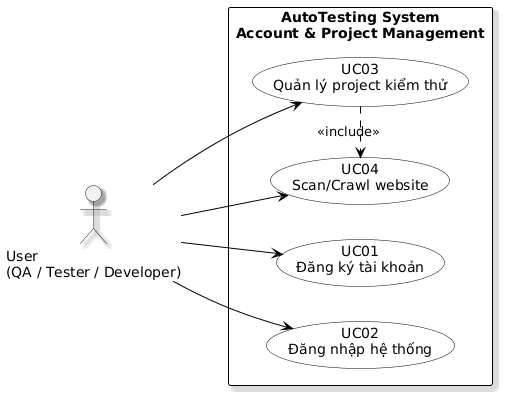
\includegraphics[
    width=0.85\textwidth,
    height=0.78\textheight,
    keepaspectratio
]{images/usecase/usecase_account_project.png}
\caption{Use case quản lý tài khoản và project}
\label{fig:usecase_account_project}
\end{figure}

Hình~\ref{fig:usecase_account_project} mô tả các chức năng đăng ký, đăng nhập, đăng nhập bằng Google, khôi phục mật khẩu, đăng xuất, quản lý project và scan/crawl website. Scan/crawl được đặt trong nhóm quản lý project nhưng là chức năng tùy chọn.

\begin{figure}[H]
\centering
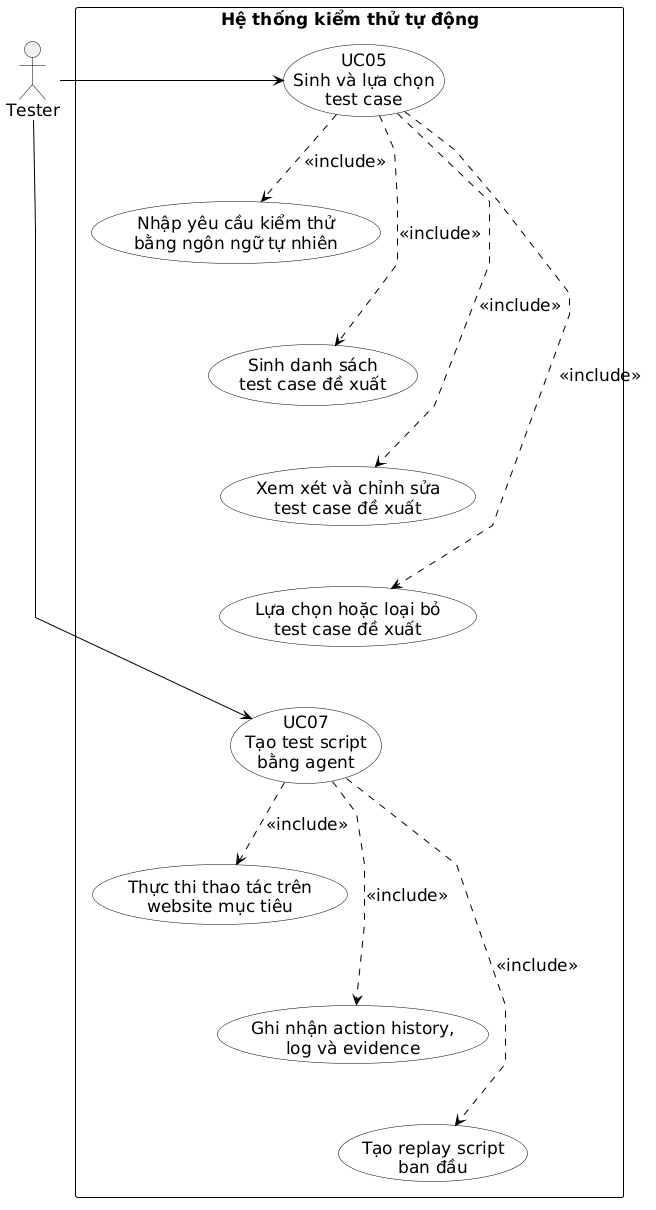
\includegraphics[
    width=0.85\textwidth,
    height=0.78\textheight,
    keepaspectratio
]{images/usecase/usecase_agent_testing.png}
\caption{Use case sinh, lựa chọn test case và tạo test script bằng agent}
\label{fig:usecase_agent_testing}
\end{figure}

Hình~\ref{fig:usecase_agent_testing} mô tả quá trình tester nhập yêu cầu tại trang \textit{Generate Testcase}, sinh danh sách test case, xem xét, chỉnh sửa và lựa chọn các test case phù hợp. Những test case được lựa chọn được sử dụng làm đầu vào cho agent để tạo automation test script.

Khi lần chạy agent thành công, hệ thống chuyển action history thành replay script để tester xem xét và xác nhận. Giao diện có thể chia thành nhiều khu vực làm việc để xử lý các nhóm yêu cầu khác nhau, nhưng các khu vực này không được tách thành use case độc lập.

Chức năng quản lý dữ liệu kiểm thử có thể được thực hiện độc lập tại module \textit{Data}.

\begin{figure}[H]
\centering
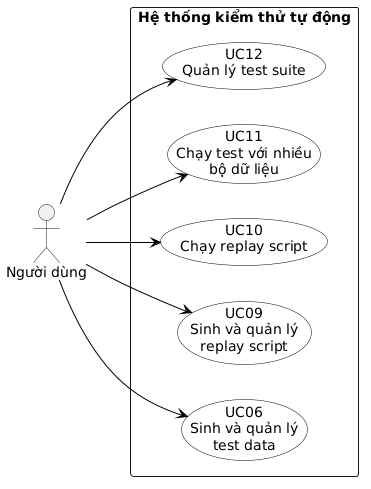
\includegraphics[
    width=0.85\textwidth,
    height=0.78\textheight,
    keepaspectratio
]{images/usecase/usecase_replay_data_suite.png}
\caption{Use case quản lý test case, replay script, dữ liệu kiểm thử và test suite}
\label{fig:usecase_replay_data_suite}
\end{figure}

Hình~\ref{fig:usecase_replay_data_suite} mô tả các chức năng xác nhận và quản lý replay script, lưu test case theo cấu trúc cây thư mục, chạy replay script với một hoặc nhiều dòng dữ liệu và quản lý test suite.

Sau khi replay script được tester xác nhận, test case cùng script được lưu tại trang \textit{Test Cases}. Tester có thể phân nhóm test case theo thư mục, module hoặc luồng nghiệp vụ để thuận tiện quản lý và tái sử dụng.

Đối với các test case đã có replay script, hệ thống hỗ trợ chế độ replay để tester sử dụng trong các lần kiểm thử hồi quy. Tester có thể quản lý test suite mà không bắt buộc phải thực hiện test run ngay lập tức.

\begin{figure}[H]
\centering
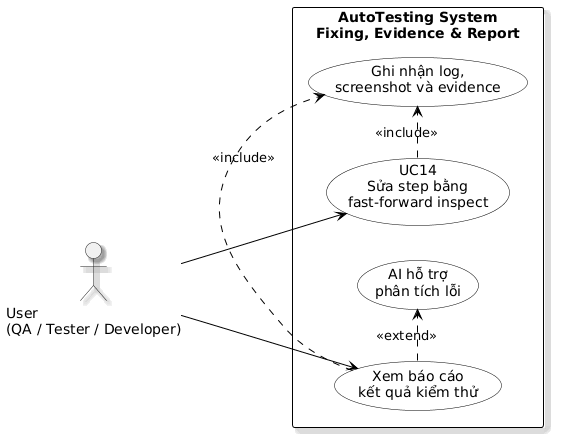
\includegraphics[
    width=0.85\textwidth,
    height=0.78\textheight,
    keepaspectratio
]{images/usecase/usecase_report_fix.png}
\caption{Use case xem kết quả và phân tích lỗi}
\label{fig:usecase_report_fix}
\end{figure}

Hình~\ref{fig:usecase_report_fix} mô tả các chức năng xem kết quả, log, screenshot, action history, evidence, report và phân tích lỗi bằng AI. Các dữ liệu này được ghi nhận hoặc tổng hợp từ quá trình thực thi test.

% =========================================================
\section{Đặc tả use case chính}
% =========================================================

Bảng~\ref{tab:main_use_cases} trình bày đặc tả rút gọn của các use case chính.

{\small
\begin{longtable}{|p{1.4cm}|p{3.6cm}|p{5.5cm}|p{3.8cm}|}
\caption{Đặc tả rút gọn các use case chính}
\label{tab:main_use_cases} \\
\hline
\textbf{Mã} &
\textbf{Use case} &
\textbf{Mục tiêu} &
\textbf{Kết quả đầu ra} \\
\hline
\endfirsthead

\hline
\textbf{Mã} &
\textbf{Use case} &
\textbf{Mục tiêu} &
\textbf{Kết quả đầu ra} \\
\hline
\endhead

UC01 &
Đăng ký tài khoản &
Cho phép người dùng tạo tài khoản mới. &
Tài khoản được tạo nếu dữ liệu hợp lệ. \\
\hline

UC02 &
Đăng nhập hệ thống &
Xác thực tester bằng tài khoản hệ thống hoặc Google OAuth. &
Phiên đăng nhập được tạo. \\
\hline

UC03 &
Quản lý project kiểm thử &
Cho phép tester tạo, xem và cập nhật thông tin project. &
Thông tin project được lưu. \\
\hline

UC04 &
Scan/Crawl website &
Thu thập sitemap và thông tin điều hướng từ base URL. &
Kết quả và trạng thái scan được lưu. \\
\hline

UC05 &
Sinh và lựa chọn test case &
Chuyển yêu cầu bằng ngôn ngữ tự nhiên thành danh sách test case có cấu trúc và cho phép tester lựa chọn các trường hợp phù hợp. &
Danh sách test case được sinh, chỉnh sửa và lựa chọn để tạo test script. \\
\hline

UC06 &
Sinh và quản lý dữ liệu kiểm thử &
Cho phép tester tạo thủ công hoặc sinh dataset bằng AI. &
Dataset được lưu để sử dụng khi thực thi test. \\
\hline

UC07 &
Tạo test script bằng agent &
Thực thi test case đã được lựa chọn bằng agent và browser automation để tạo automation test script. &
Test run, action history, log, evidence và replay script ban đầu được tạo. \\
\hline

UC08 &
Xem kết quả chạy test &
Cho phép tester xem thông tin của một test run đã thực thi. &
Trạng thái, timeline, screenshot và thông tin lỗi được hiển thị. \\
\hline

UC09 &
Xác nhận và quản lý replay script &
Cho phép tester xem xét, chỉnh sửa và xác nhận replay script được tạo từ lần chạy agent thành công. &
Test case và replay script được lưu vào cây thư mục tại trang \textit{Test Cases}. \\
\hline

UC10 &
Chạy replay script &
Chạy lại kịch bản đã lưu bằng Playwright để phục vụ kiểm thử hồi quy. &
Kết quả replay run được lưu mà không cần LLM suy luận ở từng bước. \\
\hline

UC11 &
Chạy test với nhiều bộ dữ liệu &
Chạy replay script với nhiều dòng dữ liệu đầu vào. &
Kết quả được lưu theo từng dòng dữ liệu. \\
\hline

UC12 &
Quản lý test suite &
Tạo và quản lý nhóm test case cùng cấu hình chạy. &
Cấu hình test suite được lưu. \\
\hline

UC13 &
Quản lý Object Repository &
Lưu và tái sử dụng thông tin nhận diện phần tử giao diện. &
Object và selector được lưu theo project. \\
\hline

UC14 &
Xem report và phân tích lỗi &
Xem evidence, thông tin lỗi và yêu cầu AI phân tích kết quả. &
Nguyên nhân dự kiến và hướng xử lý được hiển thị và lưu lại. \\
\hline

\end{longtable}
}

% =========================================================
\section{Kết chương}
% =========================================================

Chương này đã trình bày tổng quan hệ thống, đối tượng sử dụng, yêu cầu chức năng, yêu cầu phi chức năng và các use case chính.

Quy trình chính bắt đầu tại trang \textit{Generate Testcase}, nơi tester nhập yêu cầu bằng ngôn ngữ tự nhiên, xem xét và lựa chọn các test case phù hợp. Agent được sử dụng để thực thi các test case đã chọn và tạo automation test script. Sau khi được tester xác nhận, test case cùng replay script được lưu theo cấu trúc cây thư mục tại trang \textit{Test Cases}.

Trong các lần kiểm thử hồi quy tiếp theo, tester có thể tái sử dụng replay script thay vì yêu cầu LLM suy luận lại ở từng bước. Cách tiếp cận này giúp giảm công sức xây dựng kịch bản ban đầu, giảm số lần gọi mô hình và tăng khả năng tái sử dụng test script.

Các yêu cầu và use case được xác định trong chương này là cơ sở để thiết kế kiến trúc, dữ liệu và luồng xử lý tại Chương~\ref{Chapter4}.
